% !Mode:: "TeX:UTF-8"
% !TEX program  = xelatex
\documentclass[a4paper]{IEEEtran}
\IEEEoverridecommandlockouts
\usepackage{ctex}
\usepackage{cite}
\usepackage{amsmath,amssymb,amsfonts}
\usepackage{algorithmic}
\usepackage{graphicx}
\usepackage{textcomp}
\usepackage{xcolor}
\usepackage{listings}
\usepackage{color}

\definecolor{dkgreen}{rgb}{0,0.6,0}
\definecolor{gray}{rgb}{0.5,0.5,0.5}
\definecolor{mauve}{rgb}{0.58,0,0.82}

\lstset{frame=tb,
	language=Python,
	aboveskip=3mm,
	belowskip=3mm,
	showstringspaces=false,
	columns=flexible,
	basicstyle={\small\ttfamily},
	numbers=none,
	numberstyle=\tiny\color{gray},
	keywordstyle=\color{blue},
	commentstyle=\color{dkgreen},
	stringstyle=\color{mauve},
	breaklines=true,
	breakatwhitespace=true,
	tabsize=3
}
\usepackage[colorlinks,linkcolor=blue]{hyperref}
\usepackage[a4paper, top=2.54cm, bottom=2.54cm, left=3.18cm, right=3.18cm]{geometry}
\title{\huge{概率统计课程论文\\
		蒙特卡洛方法在积分估计上的应用}
}
\author{王凯灵 521030910356}
\begin{document}
	\maketitle
	\begin{abstract}
		蒙特卡洛积分指的是采用蒙特卡洛方法估计积分的一类算法。本文简要介绍了蒙特卡洛积分方法的理解和推导过程，分析了估计值的有效性。使用数值模拟验证了通过不同概率密度函数和样本数量得到的估计值关于真实值的趋近情况。使用蒙特卡洛积分方法估计了$\pi$值。
		\par\textbf{关键词—}
		概率论，辛钦大数定理，蒙特卡洛方法，数值模拟
	\end{abstract}

	\section{知识概述}
	\subsection{符号与缩写约定}
	\begin{table}[h]\scalebox{0.9}{
		\centering
		\begin{tabular}{c|c|c}
			\hline\hline
			符号或缩写 & 公式 & 概念 \\ \hline
			$I(f)$ & & f在[a,b]上的积分值 \\
			$pdf(x)$ & & 概率密度函数 \\
			$cdf(x)$ & $c d f(x)=\overunderset{x}{-\infty}{\int} p d f(t) d t$ & 概率分布函数 \\
			$f_u$ & & 均匀分布概率密度 \\
			$f_n$ & & 正态分布概率密度 \\
			$f_0$ & & 含0区间的概率密度 \\
			$f_s$ & & 含有无穷0的函数 \\ \hline \hline
		\end{tabular}}
	\end{table}
	\subsection{核心前备知识}
	均为课程内容以内的基本知识，此处仅作列举。
	\begin{enumerate}
		\item 概率密度与概率分布的概念。
		\item 数学期望的定义和性质。
		\item 辛钦大数定理。
	\end{enumerate}
	\subsection{蒙特卡洛方法}
	蒙特卡洛方法是一种统计模拟方法。此处我们只讨论其在积分估计上的应用。对于原函数$f(x)$在区间$[a, b]$上的积分
	$$
	I(f)=\int_a^b f(x) d x
	$$
	
	使用n个样本估计的积分值为
	
	$$
	I_n(f)=\frac{1}{n} \sum_{i=1}^n \frac{f\left(X_i\right)}{p d f\left(X_i\right)}
	$$
	
	此即为原问题的描述。直观理解上，当选择均匀分布作为概率分布函数时，当$n\to \infty$，认为样本几乎取遍所有点且分布均匀，故逼近于积分表达式。当不使用均匀分布时，为使得原函数的信息不丢失，函数应该满足在积分区间任意子区间上取值不全为0。下面给出蒙特卡洛积分公式可以估计积分值的证明。
	
	\begin{enumerate}
		\item 无偏性
		
		即需要证明：$E(I_n(f))=I(f)$。证明过程如下：
	
	$$	
		\begin{aligned}
			E(I_n(f)) & =E\left[\frac{1}{n} \sum_{i=1}^{n} \frac{f\left(X_i\right)}{p d f (X_i)}\right] \\
			& =\frac{1}{n} \sum_{i=1}^{n} E\left[\frac{f\left(X_i\right)}{p d f\left(X_i\right)}\right] \\
			& =\frac{1}{n} \sum_{i=1}^{n} \int_a^b \frac{f(x)}{p d f(x)} p d f(x) d x \\
			& =\frac{1}{n} \sum_{i=1}^{n} \int_a^b f(x) d x \\
			& =I(f)
		\end{aligned}
	$$
	
	在上面的过程中，主要使用了数学期望的定义和运算。
	
	\item 有效性
	
	即需要说明，估计的方差足够小。根据辛钦大数定理，因为
	
	$$
	E\left[\frac{f\left(X_i\right)}{p d f\left(X_i\right)}\right] = I(f) \\
	$$
	则对任意$\varepsilon>0$有
	$$
	{\lim _{n \rightarrow \infty} P\left\{\left|\frac{1}{n} \sum_{k=1}^n E\left[\frac{f\left(X_i\right)}{p d f\left(X_i\right)}\right]-I(f)\right|<\varepsilon\right\}=1}
	$$
	即，存在足够大的n使估计量无限逼近于待测量。此时，认为方差足够小。
	\end{enumerate}

	\section{目标问题与分析方法}
	蒙特卡洛积分一般用于原函数不存在或者难以给出表达式的函数积分。本例中，讲主要以函数$f(x)=e^{x^2}$为例。该函数不存在初等原函数，是连续函数。对于不分段连续函数而言，只需单独考虑某一连续区间即可。而对于离散函数，不存在积分的概念。因此，选择的函数可以代表大多数情况下的蒙特卡洛积分函数。对于处处不连续，处处不可导的一些特殊函数将在后文另作讨论。
	
	待估计量即为该函数的积分值。该函数是偶函数，此处选取的积分区间为[-3,3]，目的为选取正态分布作为概率密度函数时，可以包含原概率密度函数的主要部分。
	
	\subsection{通过概率密度生成样本的方法}
	许多代码库中均有实现相关功能，为使得原理更加清晰，本例中按如下思路实现。使用$cdf$与$pdf$的关系进行分析：首先，使用随机数表生成按均匀分布生成样本$U_1,U_2\cdots U_n$。对于样本$U_i$，求$cdf^{-1}(U_i)$。$cdf(X_i)=U_i$表示$P(x<=X_i)=U_i$，则显然有当$U_i$服从均匀分布时，$X_i$服从概率密度为$pdf(x)$的分布。
	
	\subsection{概率密度函数的选取方法讨论}
	除了可积且积分值为1的条件外，概率密度函数在积分区间上不能有取值全部为0的区间，否则在计算时，无法取到该区间上函数的值。从推导过程中看，
	$$	
		E\left[\frac{f\left(X_i\right)}{p d f\left(X_i\right)}\right]=\int_a^b \frac{f(x)}{p d f(x)} p d f(x) d x
	$$
	
	与该条件有关，如果存在区间为0，就不存在该积分式。
	
	由于积分本身与概率不相关，推测使用均匀分布$f_u$可能在收敛速度上取得比较好的效果。为了进行比较，选取了正态分布$f_n$与之对比。
	
	另外，使用概率分布
	
	$$
	f_0(x)=
	\left\{\begin{array}{lll}
		\frac{1}{3} & , & n\leq x<n+\frac{1}{2}\\
		0 & , & n+\frac{1}{2}\leq x<n+1	
		\end{array}\right.,-3\leq x\leq 3
	$$
	
	代表存在区间为0的概率密度函数。
	
	\subsection{一种特殊函数的讨论}
	$f_s(x)=\sin(\frac{1}{x})$是一个比较特殊的函数：其在本例中的积分区间上具有无穷的零点。然而，该函数是可积的，且具有非初等原函数。在考虑将其作为被积函数的同时，尝试将其作为归一化后一个概率密度函数，探究零点数量对估计效果的影响。
	
	\section{模拟方法与实现效果}
	使用python进行积分模拟。该函数在给定积分区间上的图像如图\ref{int}所示。根据自定义实现的积分运算函数，待估计量$I(f)$的标准值为2889.09025。
	\begin{figure}[h]
		\centering
		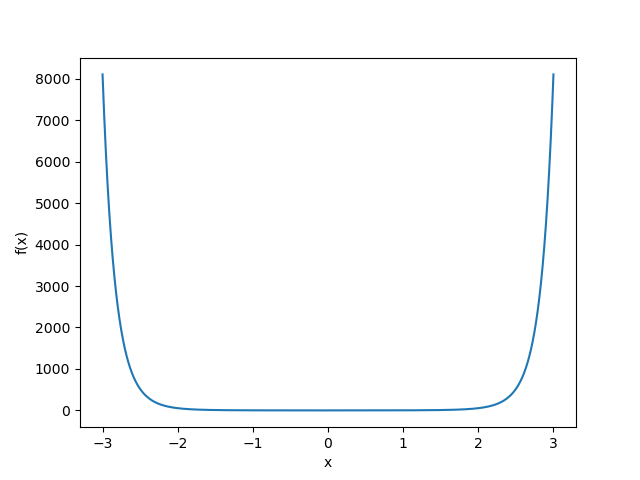
\includegraphics[width=1\linewidth]{int}
		\caption{函数在积分区间上的图像}
		\label{int}
	\end{figure}

	\subsection{样本生成方法实现}
	按照定义，实现的标准正态分布的公式。按照前文所述的方法实现了样本生成方法。考虑到要保证被积区间内样本数量一定，在原方法基础上进行调整：
	\begin{enumerate}
		\item 计算概率密度函数在被积区域上的积分值
		\item 在此基础上估计生成一定数量被积区间内的样本所需的总样本量，按该数量加量生成均匀分布样本
		\item 在求$cdf^{-1}$时，过滤不在区间内的样本，最后进行打乱，并选择所需数量
		\item 如果小概率发生过滤后样本数量不足，重新生成
	\end{enumerate}

	实际模拟生成的正态分布样本如图\ref{norm}所示。
	
	\begin{figure}[h]
		\centering
		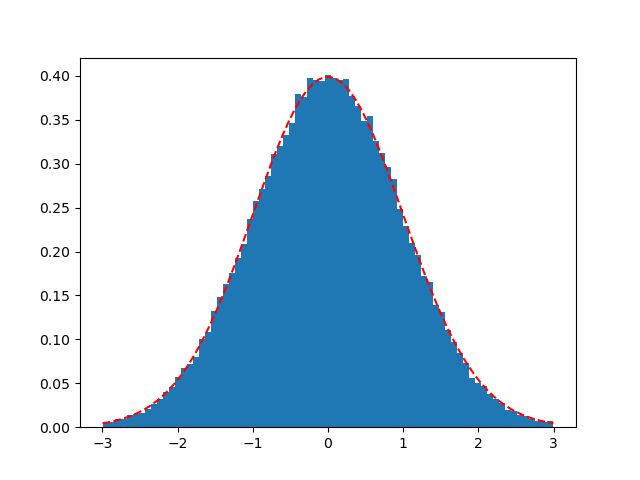
\includegraphics[width=1\linewidth]{norm}
		\caption{生成的正态分布样本}
		\label{norm}
	\end{figure}
	
	\subsection{积分模拟实验}
	使用了前文提到的四种概率密度函数，使用不同样本数量进行数值模拟。数值结果见下表。 
	\begin{table}[h]
		\centering
		\caption{使用不同密度函数的样本数量的估计结果}
		\begin{tabular}{l|l|l|l|l}
			\hline \hline
			模拟值$\backslash$样本数 & 10 & 100 & 1000 & 10000 \\ \hline
			$f_u$估计值 &7177&3015&3021&2816\\
			$f_n$估计值 &25&824&4126&2962\\
			$f_0$估计值 &439&1191&1416&1475\\
			$f_s$估计值 &96&4362&3177&2893\\\hline \hline
		\end{tabular}
	\end{table}	
	\begin{table}[h]\scalebox{0.9}
		{\centering
		\begin{tabular}{l|l|l|l|l}
			\hline \hline
			模拟值$\backslash$样本数 & 100000 & 1000000 & 5000000 & 10000000 \\ \hline
			$f_u$估计值 &2829&2896&2892&2890\\
			$f_n$估计值 &3135&2892&2869&2909\\
			$f_0$估计值 &1440&1447&1445&1444\\
			$f_s$估计值 &2872&2899&2883&2890\\\hline \hline
		\end{tabular}}
	\end{table}
	
	结合图像图\ref{vs}可以直观地观察估计值的变化趋势。
	
	\begin{figure}[h]
		\centering
		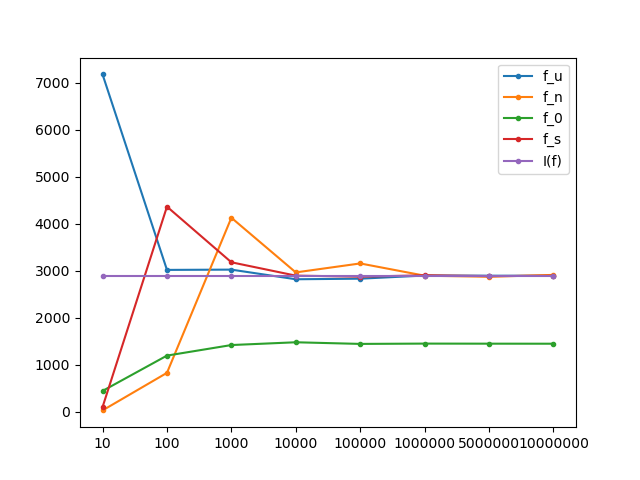
\includegraphics[width=1\linewidth]{vs}
		\caption{不同样本数量和概率密度组合的误差趋势}
		\label{vs}
	\end{figure}

	观察图线，可以发现以下信息：
	\begin{enumerate}
		\item 随着样本数量增大，各个估计值均逐渐收敛至稳定值。
		\item 在四个概率密度函数中，含有0区间的概率密度函数没有收敛到真实值，与上文提到的对于概率密度函数的要求相符。实际上，该收敛值为被积函数在概率密度函数非0区间上的积分。
		\item 在使用的4个概率密度函数中，均匀分布和含0的均匀分布收敛迅速，符合上文预期，即：使用均匀分布生成样本可能取得更好的估计效果，且具有更高的泛用性。本例中，在正态分布概率较大的区域函数值较小，所以正态分布不能取得良好效果，且估计值倾向与偏小。如果是被积函数的倒数，则估计值偏大。
		\item 使用在0点附近无线震荡的概率密度函数也可以取得良好的估计结果，即使用$f_s$进行估计。
	\end{enumerate}
	\subsection{利用蒙特卡洛积分解决实际问题}
	\subsubsection{$\pi$的估计}
	在二维平面内，使用独立的$X, Y$变量模拟二维平面里的随机点坐标，概率密度使用正态分布的概率密度。即：横纵坐标分别满足标准正态分布，积分区域为(-10,-10),(-10,10),(10,-10),(10,10)构成的矩形区域。使用该区域的目的是直接使用正态分布，不重新归一化到某一区域，方便计算。被积函数为：
	
	$$
	f(\boldsymbol x)=
	\left\{\begin{array}{lll}
		1 & , & \boldsymbol{x}^2\leq1\\
		0 & , & otherwise	
	\end{array}\right.
	$$
	
	图\ref{pi}显示了模拟结果。
	\begin{figure}[h]
		\begin{minipage}[t]{0.49\linewidth}
			\centering
			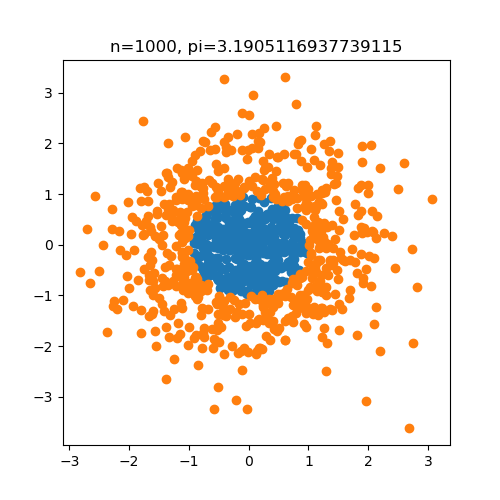
\includegraphics[width=0.9\linewidth]{pi1}
		\end{minipage}
		\begin{minipage}[t]{0.49\linewidth}
			\centering
			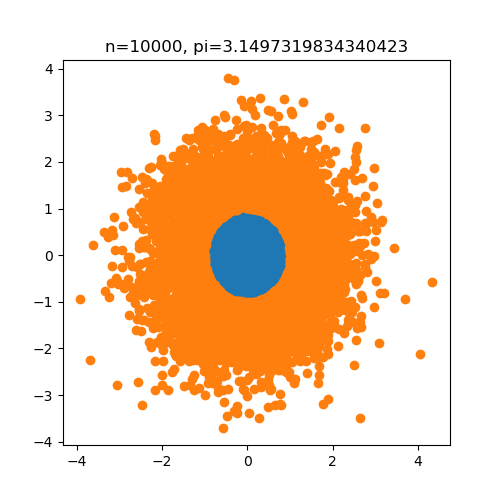
\includegraphics[width=0.9\linewidth]{pi2}
		\end{minipage}		
		\begin{minipage}[t]{0.49\linewidth}
			\centering
			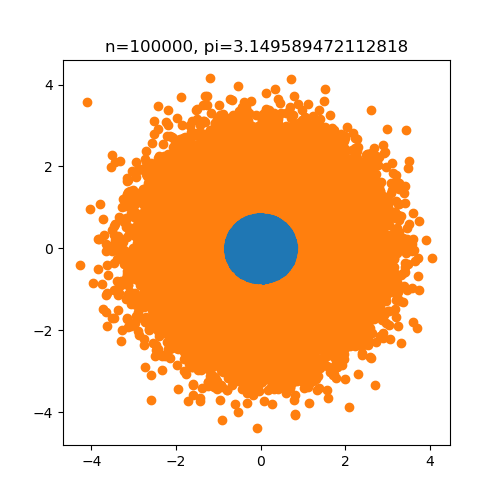
\includegraphics[width=0.9\linewidth]{pi3}
		\end{minipage}	
		\begin{minipage}[t]{0.49\linewidth}
			\centering
			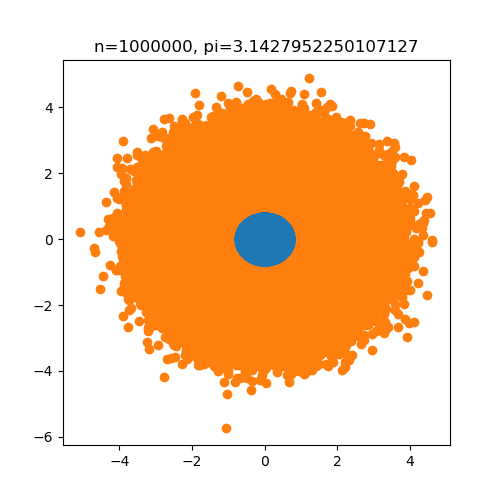
\includegraphics[width=0.9\linewidth]{pi4}
		\end{minipage}	
	\caption{数值模拟求解$\pi$}\label{pi}
	\end{figure}
	
	当样本使用1000000时，估计值达到了3.1428，已经与真实值十分接近。

	\section{高维拓展}
	蒙特卡洛方法在更高维度下，推导方法与一维类似。高维蒙特卡洛积分的形式变为
	$$
	I_n(f)=\frac{1}{n} \sum_{i=1}^n \frac{f\left(\boldsymbol X_i\right)}{p d f\left(\boldsymbol X_i\right)}
	$$
	即在高维上积分，概率密度也变为高维。实际上，在估计$\pi$值时，也可以认为使用了二维情况下的蒙特卡洛积分。
	\section{总结}
	蒙特卡洛方法估计积分值是一种十分有效的积分估计方法，只需使用服从某一概率密度的样本和样本对应的函数值即可估计积分值。即：即使函数解析式未知或无法表示，也可以通过足够多的已知点进行蒙特卡洛估计积分。当样本够多，蒙特卡洛估计值收敛于积分值。使用均匀分布可以比较稳定地进行估计，使用不断震荡的概率密度函数或正态分布，也可以进行准确的估计。实际使用时，主要取决于使用的样本服从的分布。使用蒙特卡洛积分，可以进行$\pi$的数值估计，也可以用于求解打靶问题等含积分概率问题。
	\section{附录：代码}
	\begin{lstlisting}
import numpy as np
import matplotlib.pyplot as plt


# 函数
def f_1(x):
return np.exp(x ** 2)


# 积分区间
def xr(n=1e6, l=-3, h=3):
return np.arange(l, h, 6 / n)


plt.figure()
plt.plot(xr(), f_1(xr()))
plt.xlabel('x')
plt.ylabel('f(x)')
plt.show()


# 数值积分
def numer_int(f, a, b, dx=1e-6):
res = 0
for i in range(int((b - a) / dx)):
res = res + f(a + i * dx) * dx
return res


# 样本产生
def cdf(pdf, x, dx=1e-6):
x = sorted(x)
head = 0
res = []
c = 0.5 - numer_int(pdf, -3, 0)
while head < len(x) and x[head] <= c:
head = head + 1
for i in range(int(6 / dx)):
c = c + pdf(-3 + i * dx) * dx
while head < len(x) and x[head] <= c:
head = head + 1
res.append(-3 + i * dx)
return res


def f_u(x):
if -3 <= x <= 3:
return 1 / 6
else:
return 0


def f_n(x):
return np.exp(-x ** 2 / 2) / np.sqrt(2 * np.pi)


def f_0(x):
if -3 <= x < -2.5 or -2 <= x < -1.5 or -1 <= x < -0.5 or 0 <= x < 0.5 or 1 <= x < 1.5 or 2 <= x < 2.5:
return 1 / 3
else:
return 0


f_sint = numer_int(lambda l: abs(np.sin(1 / l)), -3, 0 - 1e-6) * 2


def f_s(x):
if x != 0 and -3 <= x <= 3:
return abs(np.sin(1 / x)) / f_sint
else:
return 0


plt.figure()
_, bins, _ = plt.hist(cdf(f_n, np.random.random(100000)), bins=75, density=1)
plt.plot(bins, f_n(bins), 'r--')
plt.show()


def MC_int(f, pdf, n):
us = np.random.random(int(n * 1.2))
ns = cdf(pdf, us)
np.random.shuffle(ns)
ns = ns[:n]
res = 0
for i in range(n):
res = res + f(ns[i]) / pdf(ns[i])
return res / n


fu = []
fn = []
f0 = []
fs = []
iters = ["10", "100", "1000", "10000", "100000", "1000000", "5000000", "10000000"]
for n in [10, 100, 1000, 10000, 100000, 1000000, 5000000, 10000000]:
print(n)
fu.append(MC_int(f_1, f_u, n)), print("f_u", fu[-1])
fn.append(MC_int(f_1, f_n, n)), print("f_n", fn[-1])
f0.append(MC_int(f_1, f_0, n)), print("f_0", f0[-1])
fs.append(MC_int(f_1, f_s, n)), print("f_s", fs[-1])

realint = numer_int(f_1, -3, 3)
plt.figure()
plt.plot(iters, fu, marker='o', markersize=3)
plt.plot(iters, fn, marker='o', markersize=3)
plt.plot(iters, f0, marker='o', markersize=3)
plt.plot(iters, fs, marker='o', markersize=3)
plt.plot(iters, realint * np.ones((len(fu),)), marker='o', markersize=3)
plt.legend(['f_u', 'f_n', 'f_0', 'f_s', 'I(f)'])
plt.show()

print(fu, np.array(fu) - realint)
print(fn, np.array(fn) - realint)
print(f0, np.array(f0) - realint)
print(fs, np.array(fs) - realint)

def cdf2(pdf, x, dx=1e-4):
x = sorted(x)
head = 0
res = []
c = 0.5 - numer_int(pdf, -10, 0)
while head < len(x) and x[head] <= c:
head = head + 1
for i in range(int(20 / dx)):
c = c + pdf(-10 + i * dx) * dx
while head < len(x) and x[head] <= c:
head = head + 1
res.append(-10 + i * dx)
return res

def pi(n=100000):
nsx = cdf2(f_n, np.random.random(int(n * 1.2)))
nsy = cdf2(f_n, np.random.random(int(n * 1.2)))
np.random.shuffle(nsx)
nsx = nsx[:n]
np.random.shuffle(nsy)
nsy = nsy[:n]
res = 0
inner = []
outer = []
for i in range(n):
if nsx[i] ** 2 + nsy[i] ** 2 <= 1:
inner.append([nsx[i], nsy[i]])
res = res + 1 / f_n(nsx[i]) / f_n(nsy[i])
else:
outer.append([nsx[i], nsy[i]])
plt.figure(figsize=(5,5))
inner = np.array(inner)
outer = np.array(outer)
plt.scatter(inner[:, 0], inner[:, 1])
plt.scatter(outer[:, 0], outer[:, 1])
plt.title("n={}, pi={}".format(n, res / n))
plt.show()
return res / n


for n in [1000, 10000, 100000, 1000000]:
print(n, pi(n))

	\end{lstlisting}
\end{document}